\documentclass[10pt,twocolumn,letterpaper]{article}

\usepackage{../authorkit/cvpr}
\usepackage{times}
\usepackage{epsfig}
\usepackage{graphicx}
\usepackage{amsmath}
\usepackage{amssymb}

% Packages added by us
\usepackage{amsfonts}
\usepackage{mydefs}
\usepackage{algorithmic}
\usepackage{algorithm}

\usepackage[pagebackref=true,breaklinks=true,letterpaper=true,colorlinks,bookmarks=false]{hyperref}

% \cvprfinalcopy % *** Uncomment this line for the final submission

\def\cvprPaperID{****} % *** Enter the CVPR Paper ID here
\def\httilde{\mbox{\tt\raisebox{-.5ex}{\symbol{126}}}}

% Pages are numbered in submission mode, and unnumbered in camera-ready
\ifcvprfinal\pagestyle{empty}\fi
\begin{document}

%\title{Accelerating $\ell_1$-Minimization Using Many-Core CPUs/GPUs \\ and Application to Face Recognition
%\title{Efficient Parallelization of Sparse Representation for Face Recognition}
%\thanks{Corresponding author: . This work was partially supported by ARO MURI W911NF-06-1-0076.}}
\title{Efficient Parallelization of $\ell_1$-Minimization for Face Recognition
\thanks{Corresponding author: . This work was partially supported by ARO MURI W911NF-06-1-0076.}}

\author{First Author\\
Institution1\\
Institution1 address\\
{\tt\small firstauthor@i1.org}
% For a paper whose authors are all at the same institution,
% omit the following lines up until the closing ``}''.
% Additional authors and addresses can be added with ``\and'',
% just like the second author.
% To save space, use either the email address or home page, not both
\and
Second Author\\
Institution2\\
First line of institution2 address\\
{\small\url{http://www.author.org/~second}}
}

\maketitle

\begin{abstract}

\end{abstract}

\section{Introduction} 

%Motivate the paper by an overview about the scope and importance of $\ell_1$-minimization.
$\ell_1$-minimization is one of the most powerful tools to be added to the engineer's
toolbox in years.  It has strong theoretical motivation for both for use in recovering sparse
solutions to systems of linear equations, and has been shown to perform well even in the
presence of a combination of sparse and dense error.  Since solutions of linear systems
arise in practically every branch of engineering and there are very few application which
do {\em not} benefit from a robust error function, the applications are far to numerous to
itemize here.  
For many applications of $\ell_1$-minimization solving a system $b=Ax$, $A$ often has a
special structure that can be leveraged to compute portions of $A$ on the fly
as they are needed, speeding up perfomance of the minimization dramatically.
Unfortunately, there are many import applications where this does not hold true.
This paper targets applications where $\bb$ and $A$ contain
image data, and thus must be loaded every time they are used, as is the 
case for many problems in computer vision.
The techniques presented in this paper target these applications, as well
as others where the dictionary is dense and unstructured. $A$ must be loaded every time
it is used, and algorithm performance becomes highly dependent on memory bandwidth, rather
that arithmetic logic.

% Narrow focus for applications to Recognition Application
The primary motivating application for this paper is face recognition for access control applications.
Recently, advances in automatic face recognition have been made by re-casting
it as a sparse representation problem.  This core of this technique consists of
re-casting recognition as a sparse representation problem. This is done by  
stacking the test image into a vector $\bb$, stacking the training images for
all of the users into the columns of a matrix $A$, and solving the following
minimization problem:
\begin{equation}
\min_{\x, \e} \| \x \|_1 + \|\e\|_1 \quad \subj \quad \bb = A \x + \e.
\end{equation}
This optimization promotes a solution that is sparse both in $\x$ and $\e$. 
Sparsity in $\x$ arrises from the fact that only a subset of the training images (if any)
correspond to the user in the test image.  Sparsity in $\e$ arrises from the knowledge
that small occlusions in the test image will only corrupt a small subset of the pixels \cite{Wright2009-PAMI}.
The large coefficients in $\x$ will concentrate on the correct user, and can be used as the basis of a classifier.

For this idea to work, all of the images must be aligned. An iterative alignment
algorithm for this purpose was described as part of the \cite{Wagner2009-CVPR}, which was
the first paper to expand \cite{Wright2009-PAMI} into a functioning face recognition system.
This iterative alignment routine is based on repeatedly solving the following optimization problem:
\begin{equation}
\min_{\x, \e} \|\e\|_1 \quad \subj \quad \bb = A_k \x + \e.
\end{equation}
Where $A_k$ contains the training images for user $k$ as well as several vectors consisting of the
Jacobian of the test image $\bb$ with respect to the transformation parameters, and $\x$ contains
both the current representation coefficients, as well as an update to the transformation parameters.

\subsection{Literature review}
[Review the past parallel algorithms for $\ell_1$-minimization. Hopefully there aren't many]

[Review the available different algorithms solving $\ell_1$-minimization and $\ell_0$-minimization, please refer to Allen's SIAM paper.]
[Allen]

[Zero in and justify why we choose ALM for our implementation.]

\subsection{Contributions of the paper}

\section{Characteristics of the ALM Algorithm}
Describe the two variants of the ALM algorithm

The augmented lagrange multiplier (ALM) method utilizes a popular class of convex techniques, the lagrange multiplier, solving the problem:
\begin{equation}
F(x) = f(x) + \lambda g(x).
\end{equation}

Because the optimal lagrange multiplier values are not known, ALM iterates between estimating the solution and the lagrange multipier values.

In order to solve the recognition stage, we consider the $l_1$ problem:
\begin{equation}
\min_{\x, \e} \|\x\|_1 \quad \subj \quad \bb = A \x + \e.
\end{equation}
which can be formulated as
\begin{equation}
L_u(x,y) = \|x\|_1 + <\y, b - A\x - \e> + \frac{\mu}2 \| b-A\x-\e \|_2^2
\end{equation}

where $\mu > 0$ is a constant that penalizes infeasibility and $y$ is a vector of lagrange multipliers.

We summarize the entire ALM
algorithm as Algorithm~\ref{alg:alm}, where $\gamma$ denotes the
largest eigenvalue of the matrix $A^TA$. For the choice of parameter $\mu$, we take the same strategy as
in \cite{YangJ2009-pp} and set $\mu_0 = 2m / \|\bb\|_1$. We set $\rho=1.5$.
\begin{algorithm}[h]
\caption{\bf (Augmented Lagrange Multiplier Method Used in Alignment Inner Loop)}
\begin{algorithmic}[1]
\STATE {\bf Input:} $\bb \in \Re^m$, $A \in \Re^{m \times n}$,
$\x_1 = \mathbf{0}$, $\blamda_1 = \mathbf{0}$.
\WHILE{not converged ($k = 1,2,\ldots$)}
\WHILE{not converged ($l = 1,2,\ldots$)}
\STATE $\e_{l+1} \leftarrow \textup{shrink}\left(\bb - A\x_l + \frac{\blamda_k}{\mu_k}, \frac{1}{\mu_k}\right)$;
\STATE $\x_{l+1} \leftarrow (A^\dagger)^T \left(\bb - \e_{l+1} + \frac{\blamda_k}{\mu_k} \right) $;
\ENDWHILE
\STATE $\blamda_{k+1} \leftarrow \blamda_k + \mu (\bb - A\x_{k+1} - \e_{k+1})$;
\STATE $\mu_{k+1} \leftarrow \rho\mu_k$;
\ENDWHILE \STATE
{\bf Output:} $\x^* \leftarrow \x_k, \e^* \leftarrow \e_k$.
\end{algorithmic}
\label{alg:alm}
\end{algorithm}

In order to solve the alignment stage before recognition, we consider the $l_1$ problem: 
\begin{equation} 
\min_{\x, \e} \|\e\|_1 \quad \subj \quad \bb = A \x + \e.
\end{equation}
which is solved in a similar fashion.

We need to define the following soft-thresholding operator for a
scalar $x$ and a scalar $\alpha \geq 0$:
\begin{equation}
\textup{shrink}(x,\alpha) = \textup{sign}(x)\cdot \max \{|x| - \alpha, 0\},
\end{equation}
In practice, this operator will be applied elementwise to a vector $\x$ with a single $\lambda$,
and will be notated as $\textup{shrink}(\x,\alpha)$.

% Write about the general algorithm and then say they have to be adapted for the two problems.
% Refer to book chapter

Shown above is the general algorithm, which has been adapted for the two problems (alignment and recognition).  Refer to book...

%Show Pseudocode for one variant
%\subsection{Computational Complexity}
The Matrix-vector computions are O($mn$), and the vector-vector operations are O($m$), 
in terms of both computation cost and memory-bandwidth.  As A'A can be precomputed once, assuming the iterative solver always takes a constant number of iterations, the PALM algorithm has a computational complexity of O($mn+n^2$), where n < m.

% Complexity of entire algorithm

\section{CPU Implementation}
% With a reshuffling of the order of operations and a change of the termination
% condition, the inner loop takes the form of two matrix-vector multiplications
% and a sequence of vector-vector operations.
\subsection{CPU Hardware Parallelism}
High-level discussion of CPU parallelism, i.e.
thread-level, vector-level, cache size, cache locality
\subsection{Tuning the GEMV operation}
When matrix-vector operations are called sequentially on the same data,
the operation can be blocked so that each thread operates on the same block of data for each operation.

For Single threaded MKL sgemv, Code took          0.0335823 msec per instance to run!

For Automatic multi-threaded MKL sgemv, Code took 0.008179 msec per instance to run!

For Manually multi-threaded MKL sgemv, Code took  0.0061276 msec per instance to run!

\subsection{Tuning the Soft-Thresholding Operator}
...Make sure there are no branches

...Make sure there are no function calls

...Make sure the loop gets automatically vectorized

...Block the computation into work for different cpu cores

\section{GPU Implementation}
\subsection{GPU Hardware Parallelism}
High-level description of GPU parallelism, i.e.

The ALM algorithm requires many matrix-vector operations, this gives manycore processors such as GPUs a computational advantage for large problem sizes.  
GPUs are comprised of several streaming multiprocessors, which contain 32 floating-point units.  The GPU executes programs as SIMT (Single Instruction Multiple Threads) in groups of 32 threads called warps.  These warps are then grouped into higher levels called thread blocks and grids.  The improvement in speed comes from the memory structure of the GPU.   The GPU contains an inverted memory hierarchy so that the L1 cache stays close to the cores, providing the increase in performance.  It essentially turns the GPU from being memory-limited to computational-limited.
GPU memory also differs from CPU memory in that it requires data transfers over PCI-Express.  The cost of these transfers are amortized by doing large amounts of computation at once, requiring code to be run completely on the GPU.  The GPU can be analogous to a multi-core CPU processor, except with more sophisticated vector processing hardware.  Each streaming multiprocessor is analogous to a single CPU except that it can run multiple threads simultaneously.
All of these differences allow GPUs to perform intensive calculations such as matrix-vector operations at much faster rates than CPUs.


%You should give a brief (1-2 paragraphs) overview of the GPU architecture -- most people have heard of GPUs and what they can do by now, so it isn't worth spending a whole lot of space in the paper describing it.

%You should define the levels of the Cuda thread and memory hierarchies: i.e. warps, thread blocks, grids and register file, shared memory, global memory. Also mention that the GPU memories are all distinct from the CPU memories, and data transfers go over PCI-Express -- but the cost of those transfers are amortized by doing lots of work (i.e. solving an $\ell_1$ minimization after transferring the matrix once). It is worth spending a little space describing how the GPU is a multi-core processor (just like the CPUs), but with much more sophisticated vector processing hardware. That is: on a Fermi there are 15 cores, and each one has two 16-wide vector floating-point units.

%The GPU-algorithm is the same as the CPU algorithm: primary- and dual- ALM methods. The implementations differ in that you have to parallelize the GPU code at an additional level, and you can't use the GPU's caches to communicate between cores (only within a core). On the CPU, you only need to parallelize for the 4 or 8 cores -- and perhaps add SSE instructions when possible (usually this is inside of the BLAS library) -- any communication between cores happens implicitly via cache coherence. For the GPU, you need to parallelize for the 15 cores, but also for the 32-way SIMD parallelism of Warps. Any intra-core communication happens via the cache (aka scratchpad, or __shared__ memory) and within-block barriers (i.e. __syncthreads()), and any inter-core communication happens via the GPU's DRAM and the implicit barriers between grid launches.


cuda cores, SIMD width, scheduling restrictions, bandwidth
\subsection{Solving a Single $\ell_1$ minimization}

The GPU ALM algorithm is written in CUDA and utilizes the CUBLAS libraries.
CUBLAS are the BLAS libraries consisting of all single precision BLAS calls
which are provided by Nvidia and are optimized for GPU performance. In
addition, we coded kernel (GPU) methods for vector-vector operations to replace
operations that would have taken multiple BLAS calls. The algorithm is similar
to the CPU algorithm except that we had to parallelize the code at an
additional level. The CPU portion of the code serves as the conductor, making
calls to GPU functions and directing the flow of the code while the GPU portion
does all of the actual computation.

\subsection{Solving multiple $\ell_1$ minimizations in parallel}
This section is about Drew's kernels for solving multiple $\ell_1$ minimizations in parllel

How to efficiently perform an $\ell_1$ minimization on a single core, quote performance on a large batch.

How to solve multiple instances in smaller batches without losing concurrency, using CUDA streams.

...Mention effect of compiler verion on streams implementation

\section{Benchmarks}

In this section, we present INSERTNUMBERHERE sets of experiment to benchmark the performance
of the PALM algorithm on CPU and GPU platforms. To generate a meaningful
comparison between different hardware architectures, we compare on a per-board
basis:  For CPU implementations, the benchmark makes use of as all of the cores
in as many cpu's are present.  For GPU implementations, the benchmark makes the
best use of the entire GPU chip (most GPU boards have a single GPU chip). Both
implementations utilized single precision floating point datatypes and were
verified to output results differing by no more than $10^{-4}$.

To construct the benchmark for synthetic data, we first created an $m \times n$
matrix $A$ with entries $\pm 1$ each with a $50\%$ chance.  Then we created a
sparse vector $\x_0$ with $k\%$ nonzero random entries.  We also created a
sparse vector $y_k$ with the same number of non-zero entries as $\x$.  Let
$\y_0 = A \x_0 + \y_k$.  We timed the time taken for the ALM algorithm using
$\y_0$, $A$, and other inputs.  The other inputs included, maximum number of
inner/outer loop iterations, and inner/outer loop tolerance level.
% give a discusison of how to construct the benchmark: one paragraph for
% protocol on how to construct synthetic data second P for protocol on how to
% construct the face data


\subsection{PALM $\ell_1$ minimization benchmark on Synthetic Data}

In this section, we benchmark the performance of MATLAB, BLAS MKL, and GPU CUDA
implementations of the Primal ALM algorithm on synthetic data to find at which
point the GPU implementation runs faster than CPU implementation.  To simply
the benchmark, we cap the number of inner iterations at 50 and outer iterations
at 5000 and run the algorithm to convergence.  CPU code was run on an Intel
Dual Socket Quad Core with 8 gigs of DDR3 RAM.  GPU code was run on a GTX480 We
ran the A matrix with different ratios between m:n from 10:1:5 for
m:2000:25:8000 with an x vector of 10 percent sparsity.  Tolerance levels were
empirically seen to allow best performance with the inner loop tolerance set at
one order of magnitude lower than the outer loop tolerance.

Results were plotted as total size of A and A'A vs Gb/s and size of A vs time
elapsed to run a single $\ell_1$ solver.

%An example of image inclusion for Victor:
\begin{figure*}
\centering
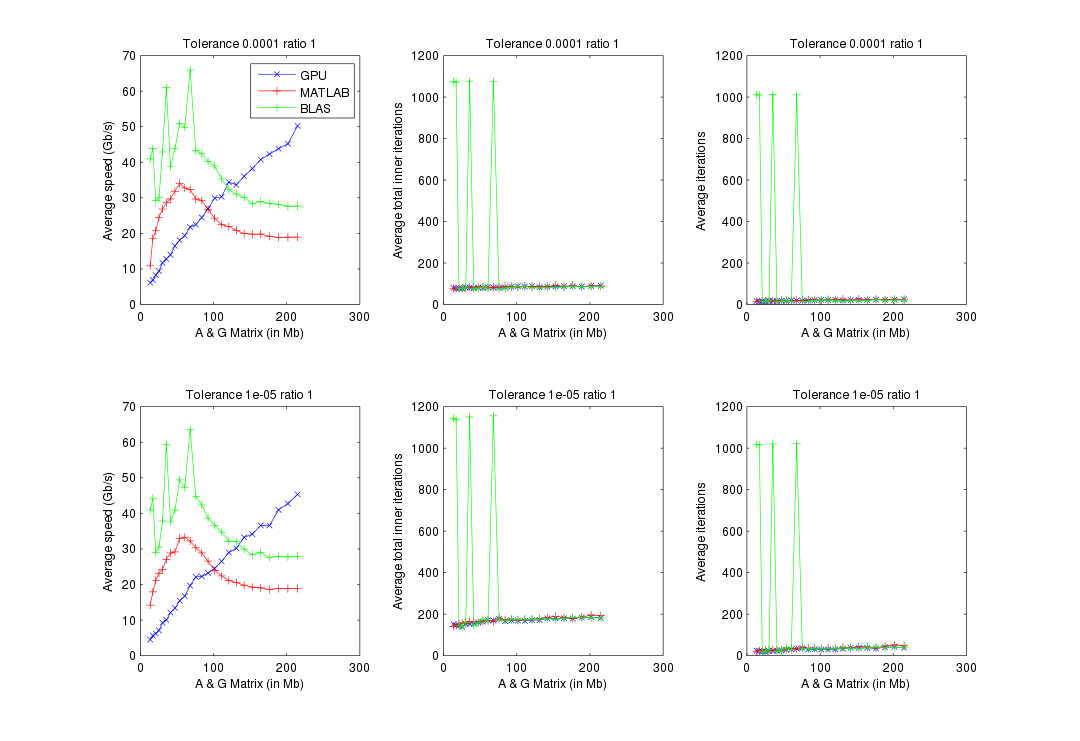
\includegraphics[width=3.5in]{figures/PALM_benchmark_ratio_1.png}
\caption{This is where the caption goes.}
\label{fig:uniqueidentifierforthisimage}
\end{figure*}

% change picture to only include CPU/GPU not MATLAB

As the dimensions of A increase, so does the significance of the size of AtA.  Until the A and AtA matrix reach x Mb, the CPU version runs faster than the GPU.  

\section{Conclusion}
...How lessons from this paper extend (or don't extend) to other similar problems in computer vision

...Reiterate how the appropriate hardware choice depends on the problem size.

{\small
\bibliographystyle{../authorkit/ieee}
\bibliography{faces}
}


\end{document}
